% !TEX TS-program = pdflatex
% !TEX encoding = UTF-8 Unicode

% This is a simple template for a LaTeX document using the "article" class.
% See "book", "report", "letter" for other types of document.

\documentclass[11pt]{article} % use larger type; default would be 10pt

\usepackage[utf8]{inputenc} % set input encoding (not needed with XeLaTeX)

%%% Examples of Article customizations
% These packages are optional, depending whether you want the features they provide.
% See the LaTeX Companion or other references for full information.

%%% PAGE DIMENSIONS
\usepackage{geometry} % to change the page dimensions
\geometry{a4paper} % or letterpaper (US) or a5paper or....
%\geometry{margin=1in} % for example, change the margins to 2 inches all round
% \geometry{landscape} % set up the page for landscape
%   read geometry.pdf for detailed page layout information

\usepackage{graphicx} % support the \includegraphics command and options

% \usepackage[parfill]{parskip} % Activate to begin paragraphs with an empty line rather than an indent

%%% PACKAGES
\usepackage{booktabs} % for much better looking tables
\usepackage{array} % for better arrays (eg matrices) in maths
\usepackage{paralist} % very flexible & customisable lists (eg. enumerate/itemize, etc.)
\usepackage{verbatim} % adds environment for commenting out blocks of text & for better verbatim
\usepackage{subfig} % make it possible to include more than one captioned figure/table in a single float
% These packages are all incorporated in the memoir class to one degree or another...

%%% HEADERS & FOOTERS
\usepackage{fancyhdr} % This should be set AFTER setting up the page geometry
\pagestyle{fancy} % options: empty , plain , fancy
\renewcommand{\headrulewidth}{0pt} % customise the layout...
\lhead{}\chead{}\rhead{}
\lfoot{}\cfoot{\thepage}\rfoot{}

%%% SECTION TITLE APPEARANCE
\usepackage{sectsty}
\allsectionsfont{\sffamily\mdseries\upshape} % (See the fntguide.pdf for font help)
% (This matches ConTeXt defaults)

%%% ToC (table of contents) APPEARANCE
\usepackage[nottoc,notlof,notlot]{tocbibind} % Put the bibliography in the ToC
\usepackage[titles,subfigure]{tocloft} % Alter the style of the Table of Contents
\renewcommand{\cftsecfont}{\rmfamily\mdseries\upshape}
\renewcommand{\cftsecpagefont}{\rmfamily\mdseries\upshape} % No bold!

%%% END Article customizations

%%% The "real" document content comes below...

\title{CS7091 - Industrial Internship Midpoint Report}
\author{173324649 - Efeosa Louis Eguavoen}
%\date{} % Activate to display a given date or no date (if empty),
         % otherwise the current date is printed 

\begin{document}
\maketitle

\section{SMART Goals}
For the course of my Internship, I decided to set myself a mixture of both technical goals and soft goals. I decided this as I thought my growth as an engineer is not only bound by the depth of my technical skills but also by my soft skills as I need to develop my interpersonal skills also.

\subsection{Technological Goals}
\subsubsection{Goal 1: Learn 1 new technology in asynchronous programming and successfully implement it in a task.}
\textbf{Specific}: This goal is specific to my development as an engineer as I feel this is an area I'm unfamiliar with as I haven't used it at all in my college work.  This is something that I wish to work on during the course of my internship so I can improve my level of skill in this area and thus strengthen my engineering skill as a result. 
\\ \textbf{Measurable}: This goal can be measured by the completion of a pull request to the main code base in which I have utilised a technology in asynchronous programming in the code I have written. 
\\ \textbf{Achievable}:This goal is achievable as from talking with my team lead,  our team uses asynchronous process in the code base we're responsible for,  so completing this goal should be within the scope of my internship.  There are numerous asynchronous technologies that are deployed in Hubspot so for me to complete this goal, I should be able to achieve this with the help of my team.
\\ \textbf{Relevant}: The relevance of this skill is that companies often have to deal with tasks asynchronously due to the fact they may take quite some time to complete,  so we can't let our code just hang while it completes.  Improving my skill in this field is definitely of benefit to me as an engineer as it makes me more well rounded. 
\\ \textbf{Time Bound}: This goal can be completed as soon as I'm given a task that requires me to use asynchronous processes.  I have set myself a deadline of the end of April to complete this goal. 
\subsubsection{Goal 2: Develop my coding style to be compatible with the world of work to reduce time how long my pull requests are in review by understanding the coding practices at Hubspot}
\textbf{Specific}: This goal is for me to improve my coding style and the way I code to be more professional in nature and thus more compatible with the world of work. This goal is specific as I've specified why I wish to achieve this and how this can be achieved. 
\\ \textbf{Measurable}: This goal is measurable by comparing the length of time it takes for my pull requests to be merged to the main code base.  This goal can also be measured by the number of comments pertaining to coding style in pull requests changing.
\\ \textbf{Achievable}:This goal can be achieved as there's a document at Hubspot of coding practices and architectural patterns to be deployed when coding.  By my reading,  understanding and most importantly,  implementation of this document I can achieve this goal.  My team members reinforcement on maintaining these standards in day to day work and pull requests can help me achieve this also.
\\ \textbf{Relevant}: This is a relevant goal to have as the readability and maintainability of a code base is very important especially when a codebase grows in size and becomes more and more difficult to pay off the technological debt.  We can help avoid this somewhat by maintaining standards and practices in how we should code,  to reduce the amount of time necessary to maintaining legacy code and increase the ease of understanding of people that may reuse your code later.
\\ \textbf{Time Bound}: This goal is something that I'll continuously be working on over the course of my internship.  I've set myself a deadline of the end of my internship to be able to fully incorporate the coding style.
\subsection{Soft Goals}
\subsubsection{Goal 1: Be able to receive feedback and also give back constructive feedback in order to increase my growth as an engineer by giving me instruction in areas I may be lagging behind, whilst being able to give my team lead direction in how best I learn and thus grow}
\textbf{Specific}: This goal is related to how I receive feedback as an engineer and how I take the feedback,  whilst also being able to support my growth as an engineer by giving me team lead instruction in how best I learn as an engineer so that can be accommodated to increase my growth in turn. 
\\ \textbf{Measurable}:This goal is measurable through the feedback I receive from my team lead.  Measuring soft skills is often more difficult as they aren't as easily quantified,  but for this specific goal it can be measured via the feedback I receive from my team lead in terms of how I've acted given previous feedback and how I've implemented previous feedback.
\\ \textbf{Achievable}: This is an achievable goal as I have weekly 1:1's with my team lead to discuss things and see how I'm getting along.  Through these 1:1's I can get and give feedback frequently enough that I can achieve this goal. 
\\ \textbf{Relevant}: This skill has plenty relevance as an important aspect of growth is via taking feedback and implementing this feedback to plug the holes so to speak.  Equally,  being able to give quality feedback can be very important as you can help nurture those around you and show those around you the best way to interact with you to fast track your growth as we all learn differently and thus need different styles of interaction.
\\ \textbf{Time Bound}: This goal is something I will continuously be working on thorough the course of my internship as learning to take feedback and giving good constructive feedback requires a long time to learn how to do well. 
\subsubsection{Goal 2: Increase my networking skills by having at least 10 1:1's with people on and outside my team to widen my network and learn more about other people's progression in Hubspot}
\textbf{Specific}:The goal here is to increase the amount of people I know in the industry by talking and interacting with numerous people in Hubspot and learning about the path they took to reach the different roles and such they've gained. This goal is specific to me ability to network and narrowed down to an essential part of networking,  talking to new people. 
\\ \textbf{Measurable}: This goal is measurable in the amount of 1:1's and new connections I succeed in making over my time in Hubspot.  If I can successfully have at least 10 1:1's with different people in Hubspot,  I think I'll have achieved my goal of increasing my networking skills and also widening my network.
\\ \textbf{Achievable}: This goal is achievable as in Hubspot there are multiple slack channels dedicated to arranging 1:1's coffee chats with anyone that's interested in partaking.  Also,  my team lead can assist me in arranging meetings with engineers and team leads on other teams also.
\\ \textbf{Relevant}: This goal has relevance as whilst your technical skill as an engineer is important,  it's difficult to show how good an engineer you are when you meet someone for the first time.  Instead the most important skill here is how you network and how well you are able to sell yourself.  Also, by talking to people that have been in the industry for a while,  you can learn from them and their mistakes to streamline your progression in your career. 
\\ \textbf{Time Bound}: I intend to complete at least one 1:1  a week between now and the end of my internship which should total to more than 10.  I've set myself a hard deadline of the 2nd week of May. 
\section{Reflective Diary}
\subsection{Week 1}
For the first week, we were focused mainly on getting setup. We went through numerous onboarding workshops the first week to teach us about the HubSpot product, the different aspects of the HubSpot product and a general introduction to our different departments. During the first week, I also met with my team lead, Gary MacElhinney and we talked a little about our team and what products we own and maintain. I created a slack channel to talk with my fellow interns and such in the first week also as there wasn't many engineering interns in total so I thought it'd be a good idea to keep in touch. 
\\\\ 
Reflection: At the time the onboarding felt somewhat un-necessary, but looking back at it now, it gave me a lot of context into what HubSpot actually is and why the work I do normally is important. Starting in a pandemic definetly affected how I felt about the whole onboarding as I felt somewhat disconnected from the rest of the interns but making the intern channel helped subside this feelings. 
\subsection{Week 2}
This week was more focused on the engineering side. We were given an engineering project that would introduce us to all the different tools and processes HubSpot uses in their engineering teams. The project had both a mixture of front end and back end development so we got to interface with the whole stack. I also got to meet the other members of my team and get a more indepth explanation of the repositories and such that we own. As part of the onboarding project, the final task is to send out a newbie intro - essentially an email about yourself that includes a link to do a 1:1 with anyone that's interested. Due to this, I got a chance to have a meeting with another engineer in the Chicago branch of Hubspot. 
\\\\
Reflection: The onboarding engineering project was very dense and a little confusing at the time. I felt I could've completed it quicker if I had asked for help quicker and not spent so much time trying to figure stuff out myself as I had a team to rely on. But I now reference the onboarding project all the time as now those tools I was introduced to have more context of their usefullness and how to implement them. Doing the 1:1 with someone not on my team was great and helped me to grow my confidence and move towards accomplishing my goal of growing my network.

\subsection{Week 3}
This week I was assigned my first actual task. My task was to implement a utility class to create a standardised way to output multicurrency codes as we need to make multicurrencies more standardised to complete a large project of making items and such imported from other companies editable within HubSpot. To complete this task, I learnt about dependancy injection and Guice, a technology that allows us to do dependancy injection. I did a team tech talk on blockchain and decentralised finance in front of my entire team this week also. On Friday after work, our team played some video games together so we could get to know each other better.
\\\\
Reflection: The first task was rather daunting as learning about a new complex system whilst trying to code in a way to reduce future maintenance whilst maintaing readability was difficult. I felt like I didn't communicate as best I could to get myself unblocked and moving forward as I didn't want to ask silly questions. If In could change anything I would've asked more questions and taken more time to learn about the tools available to me to help me get unblocked. Doing the team tech talk was very important for me to increase my confidence in public speaking but also teaching my team about new technologies felt like I was having some real input. The team bonding on the Friday really went a long way to increasing my familiarity with my team mates and helped me understand the culture more at HubSpot.
\subsection{Week 4}
This week I created my first pull request for my inital task. There was a lot of comments and feedback about my code from my team that I spent most of the week working through so the code would be in a good state that it could be merged, especially There's a big emphasis on test driven development in my team so there was numerous iterations and testing involved before the code was in a good state. I also finally met with the manager of my team, Ricky. 
\\\\
Reflection: The whole PR process felt kind of personal initally as my code was under a lot scrutinzed. But I realized now that the whole point of the intense scrutiny isn't to knock you down but to encourage better coding practices such as consistent naming of parameters, utilizing certain design patterns and thorough testing to prevent unseen bugs as when the code goes to production, it can affect customers negatively which should be avoided as much as possible. 

\subsection{Week 5}
This week I moved onto my next task. As part of our teams future mission, we need to standardise fields across the products we own. As a part of this, we need to standardise when a new multi-currency gets added to a person's account and how this is represented. To do this I needed to add learn a new technology in asynchronous programming, Kafka and create a new Kafka consumer. (Go more into depth about this later). This week I also had my monthly review with my team lead Gary. We discussed about some of my strong points such as asking questions and being willing to take on new tasks and such. He also gave me some areas to improve on such as being more forthcoming with updates on my issues and becoming more independant in my work by being able to find the answers to my questions myself.
\\\\
Reflection: The review gave me some really actionable feedback. The positive feedback helped me reinforce those traits, whilst the constructive criticism helped me to see some of my flaws. I realised that since I'm more used to work by myself, I tend to go off for hours and code and then just present when I'm done, which is against our teams motto of building together. Keeping the other members of your team in the loop of what you're doing is advantageous as they can suggest approaches you may not have thought of and can also see mistakes you're making as you're making them, which reduces on time in PR. As a result of this, work can be done quicker resulting in a higher turn over of work in a period of time.

\subsection{Week 6}
At the start of this week, I was asked to pivot from working on the multicurrencies to working on Hublets based work as out team was currently in Code Red(Maintenance mode essentially) and our team was trying to exit it as soon as possible to work on new features instead. Currently all data goes through the North America data centres but as part of GDPR, customers have the right to chose if their data can leave the US. Also there's high latency for requests as they have to travel so far to get a response. This is where Hublets come, they help solve GDPR concerns whilst also reducing latency. The task I was given was to redo all the webhooks for Shopify to target a new load balancer that would then redirect the data to the right Hublet, be it the one in North America or Europe. To complete this job I had to write a backfill job which is comprised of 2 main parts; fixing all the old data and then changing how any new data is created. I learnt about Jackson, a json processor for java that can create classes and such for from templates that you create. This helps to standardise the code and reduce the amount of future work necessary as classes are auto-generated from your templates. 
\\\\
Reflection: Taking on the feedback from the previous week definetly helped me to increase the rate at which I worked on this task this week. Initally it was hard pivoting from one task to another but my team helped me to gain a footing in the Hublets work as they had been working on it for some time. Leaning on your team and using them as a resource is incredibly useful and helped me to be able to make progress much quicker than if I had done what I was doing before and just coding by myself and not giving updates and such. They unblocked me when I provided regular updates to my issues and we did some pair programming work when necessary. An efficent team can certainly increase the productivity of yourself as an engineer as multiple people working in collaboration can always solve problems much quicker than if you were working on something by yourself.

\newpage
\section{Technology Management Processes}
At HubSpot there are multiple process in place to manage the software engineering process.
\subsection{Project Management Methods}
The actual methodology in place tends to vary on a team by team basis. The technical lead(TL) for the team usually tries to find what works for the team and then adapt a strategy based off this. 
\\ In regards to the team I'm working with, our style is the hybridization of the agile and scrum style of project management. The work for our team is broken up into 2 week sprints where at the beginnig of a new sprint, we look at our issues and then assign tasks as necessary to be done over the next 2 weeks. This works for our team as we work on multiple different repositories and projects so we need a little more flexibility than a traditional waterfall style of management would give us. Our team sometimes may hve to switch tasks to deal with certain situations that might arize called Crit-Sits where we need to down tools and focus on fixing an issue that is currently impacting customers. These issues can be quite complex to solve and require a lot of time to fix so this style of management help us be able to pivot to new tasks quickly as we can pivot from whatever we were doing to something else entirely as our sprints are short enough that we can reprioritize without having the adverse affect of being too behind schedule. In terms of when we have meetings to discuss what tasks need to be done and the current progress of tasks, we have daily stand ups at different times depending on if we're meeting with our PM who's in the United States. In terms of long term management of projects, a group called the triad is responsible for the long term vision of our team.
\\ We also have 2 other weekly meetings to discuss our systems: \begin{itemize} \item \textbf{Backlog Grooming}: This is a weekly meeting to asses the state of the major systems our team oversee and see if any of them require any major maintenance to be done due to unusual levels of downtime and such. \item \textbf{Ops Review}: This is another weekly meeting we hold with our PM to see what issues we have on our board. We use this meeting to reasses our priorities and shift focus to other things if necessary. \\ \end{itemize} 


\subsubsection{\textbf {Strengths and Weaknesses}}
This approach to management has it's strengths and weaknesses of course.
\\
Positive Effects \begin{itemize} 
\item The allure of such a stratedgy is it allows for rapid development and iteration of projects and such and allows for members on the team to be constantly working on something new and interesting, which in turn reduces employee turn over as teams aren't stuck doing the one thing for extended periods of time. 
\item The rapid prototyping and development of features fits well with the HubSpot philosophy of moving fast and efficently. 
\item The added visibility of tasks and such is also a major benefit through scrum meetings/stand ups. 
\item Feedback from management and customers can quickly be integrated.
\end{itemize}  

\subsubsection{\textbf{Negative Effects}}
 \begin{itemize}
 \item Scope creep can become a problem as more features and ideas can be suggested and implemented as there no set end date.
 \item Assuring the quality of code can be difficult unless there's a large empahsis on testing
 \item Adopting this methodology in large teams can be unwieldly and messy.
\end{itemize}
HubSpot usually has small teams of no more than 5 engineers which prevents the messiness that comes with doing this in large teams. Also there's a rather large emphasis on testing at HubSpot to prevent bug filled code being in production. When a bug is found in production and it affects multiple customers, it triggers a Crit-Sit which forces the team responsible to switch to fixing that bug. A post mortem is then also done to discuss what caused the bug, how it can be prevented in future and how it occured in the first place, without any blame being placed on an individual. This process gives teams an incentive to write clean code. \\\\Scope creep can become a problem at times, especially if it's for a major feature. To combat this, having well defined parameters of the base functionality of new features should be declared before any coding is done, and as progress is done on the feature, keeping in constant reference to the core functionality can be useful in preventing scope creep by enabling those working on new features the ability to see when un-necessary things are being added that aren't within the original defined parameters.
\subsection{Team Structures}
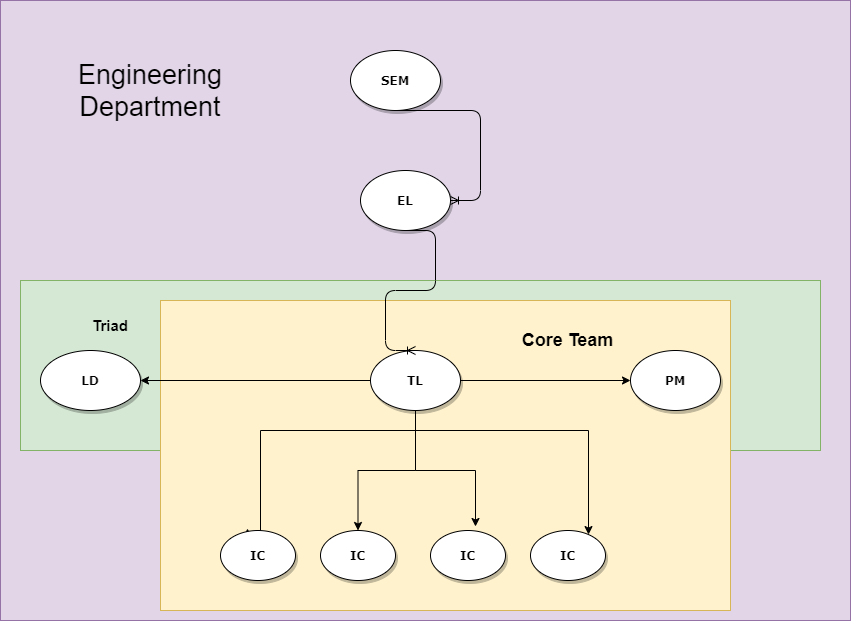
\includegraphics[scale = 0.5]{Team Structure.png}
The above image is an image of the team structures in place at HubSpot.
\subsubsection{\textbf{Roles and Responsibilities}}

\textbf{SEM -  Senior Engineering Manager}
\begin{itemize}
	\item Responsible for leading Multiple Teams and Engineering Leads
	\item Engineering Leads and Technical Leads report back to them directly
\end{itemize}
\textbf{EL -  Engineering Lead}
\begin{itemize}
\item Responsible for leading a small set of teams
\item Midpoint between Tech Lead and Senior Engineering Manager
\item Technical leads report to them
\end{itemize}
\textbf{TL -  Team Lead}
\begin{itemize}
\item Responsible for leading a team of individual contributors
\item Responsible for defining and sharing goals and challenges for the team
\item Helps to grow the skills of engineers in their team, both technically and interpersonal
\end{itemize}
\textbf{PM -  Program Manager}
\begin{itemize}
\item Works alongside Team Leads to provide solutions to customer problems
\item Can be on multiple teams/own multiple products
\item Responsible for creating with the TL goals and guardrails for their product
\end{itemize}
\textbf{LD -  Lead Designer}
\begin{itemize}
\item Responsible for the Front End Team
\item Discuss implications in terms of UI/UX for possible new features
\end{itemize}
\textbf{IC -  Individual Contributor}
\begin{itemize}
\item Part of a team of 3-5 engineers
\item Reports to a Team Lead
\item Provides feedback on tasks for the team and possible implementations of said tasks
\end{itemize}
From the above image, we can see how the different team structures fit into each other. On the largest level, the \textbf{Engineering Department}, the Senior Engineering Manager oversees the whole department. Under them are Engineering Leads and Team Leads. 
\\\\
From there is the \textbf{Triad} who are in charge of discussing the long term vision of an individual team. 
\\\\
Finally there's the \textbf{Core Team} of individual contributors being lead by a Team Lead and a Program Manager.

\subsection{Tools}
At HubSpot we use a large variety of tools to manage the numerous engineering processes a team might have to manage. Tools can largely be split into 3 main categories: \begin{itemize} \item Communication \item Engineering \item Management \end{itemize}
\subsubsection{\textbf{Communication Tools}}
\begin{itemize}
\item Slack\\\\

\includegraphics[scale=0.07]{slack.png}
\begin{itemize}
\item This is the primary means of communication we use at HubSpot
\item Each team has their own respective slack channels and then there's channels for each step up the hierarchy.
\item Slack is also used to ask questions to other teams as channels are open for people to jump in and out of.
\end{itemize}
\item Zoom\\\\

\includegraphics[scale=0.2]{zoom.png}
\begin{itemize}
\item This tool is used primarily to hold meetings and such within and between teams due to the fact that the entire company is remote.
\item We also use slack to do pair programming and debugging sessions within my team as some issues require more instantaneous communication than talking on slack can provide.
\item On team I'm working on,  we also have an ongoing zoom call that is meant to simulate the workspace as we are all on the meeting during the workday so we can reach out for help when we need it.
\end{itemize}
\item G Suite \\\\

\includegraphics[scale=0.1]{gsuite.png}
\begin{itemize}
\item G Suite is used primarily to write up documents and such for future plans we have for different products
\item We also use the G Suite in re-mediation meetings following a Crit-Sit to discuss what went wrong, what caused the issue and what we can do to prevent it in future.  
\end{itemize}
\item Jira \\\\

\includegraphics[scale=0.14]{jira.png}
\begin{itemize}
\item Jira is the software we use to manage customer issues about certain parts of our product
\item Initially,  a customer opens a jira and is assisted by the customer support team,  but when an issue is sufficiently complex that it can't be solved by them,  it gets passed on to the engineering department.
\item If more than 5 Jiras remain open pertaining to a certain aspect of our product,  this triggers a Critical Situation or Crit-Sit. 
\end{itemize}
\item Slack Bots
\\ At HubSpot,  there's a number of different Slack bots we use to help inform us of any sort of communication that happens on other platforms we may not as actively manage manually.
\begin{itemize}
\item Hedwig: This bot helps us monitor new comments on our issues as well as comments made to pull requests.
\item Orion: This Bot primarily informs us of about the build status of different repositories. It sends a message to who ever is the owner of the most recent push to our GitHub about the status of the build whenever it changes. 
\item PI Bot: This bot gives us insight into currently running Jobs.  When a job runs and fails or finishes, it sends a message to who ever initiated the job about it's status. 
\item JiraHub: This bot sends a message to which engineer is assigned a Jira and also when there's an update on the Jira,  such as a comment from other engineers  or contact from the customer support team. 
\end{itemize}
\end{itemize}
\subsubsection{\textbf{Engineering}}
\begin{itemize}
\item Blazar\\\\
Blazar is used to monitor and run different builds of Github Repositories. Blazar only builds the part of the repository that have changed when a commit is pushed . It reports back to Orion on the status of a build using GitHub Webhooks.
\item Singularity
\begin{itemize}
\item Singularity is the software we use to manage running jobs. 
\item Jobs are processes that often only do one thing such as fix data in customer accounts.
\item When a job runs and the status of it changes,  a message is sent to the person who initated the job via a slack bot. 
\end{itemize}
\item Github \\\\

\includegraphics[scale=0.2]{github.png}\\\\
GitHub is what we use to manage our code base and for version control of our code base also.  There are multiple repositories in HubSpot that all belong to different teams. 
\end{itemize}
\subsubsection{\textbf{Management}}
\begin{itemize}
\item Kepler \\\\
Kepler is used as an overview of all our systems,  code,  jobs and alerts.  We use this as the first port-of-call for all our systems as we can see the current status and manage them directly via the dashboard.  Kepler also provides numerous metrics for our systems such as downtime, accesses and the current network traffic.
\item 15Five \\\\
15five is continuous performanve management software that is used at HubSpot to manage and track the goals and performance of employees. Every week, employees fill out their goals and objectives for the week and then at the 1:1 meeting with their TL, these goals are discussed. 15five also can be used to give feedback to employees on their performance.
\item Orion
\begin{itemize}
\item Orion is the primary tool we use for deploying and managing builds of code. 
\item When an engineer pushes some code to GitHub,  a new build is triggered in Orion.  Using the integrations built into slack,  a message is sent to the engineer if the build fails and when the state of a build changes also.
\item Orion is also used to manage when we push code to QA and production.  When a pull request is closed,  a build is usually pushed to QA to be tested further and see what kind of behaviour could occur if it were to be pushed to Prod. 
\item If it passes all extra testing in QA,  it is then pushed to Prod. 
\end{itemize}
\end{itemize}
\textbf{Tool Optimizations} \\\\
A wide array of tools are used at HubSpot to manage a menagerie of microservices and such. But the sheer number of tools can be rather overwhelming as to what to use for what service. Some possible suggestions I would propose to reduce complexity would be: 
\begin{itemize} 
\item Reducing the number of tools overall and compartmentalizing the tools to what services their most relevent for. At the moment, tools are strewn around somewhat and often deciphering the correct tool to use can be a bit of a minefield. By reducing the tools used and specifying what they should be used for, this can be avoided or at the very least reduce the learning curve. 
\item There's an onboarding at the moment that introduces you to the major tools used as an engineer but it fails to really deliver how best to use these tools accordingly. To help with this, a kind of auxiliary onboarding teahing how best to use your tool according to your department would be helpful.
\end{itemize}
\subsection{Processes}
 \begin{itemize}  
 \item Our TL and our program manager(PM) come together with the lead designer to discuss what's the next milestone or objective for our team and thn decide what are the major deliverables necessary to make this a reality. 
 \item From there these major deliverables are then broken down into smaller deliverables by our TL and PM and brought to the team. These smaller deliverables are then discussed with the team to see what needs to be done first and what blocks other work that needs to be done. 
 \item Issues are then created for each of these individual tasks and are added to our ZenHub board. Some issues may be tagged as investigations if it's not immediatly clear what work needs to be done in order for the issue to be closed, whilst others may be flagged as implementaions, where the team may need to get together to discuss how's the best way to implement more complex features and such.
\\ \end{itemize}
\subsection{Communication Strategies}
\end{document}
